\section{Day 21: Coverings (Nov. 19, 2024)}
Outfit of the day: the look speaks for itself
\begin{figure}[h]
    \centering
    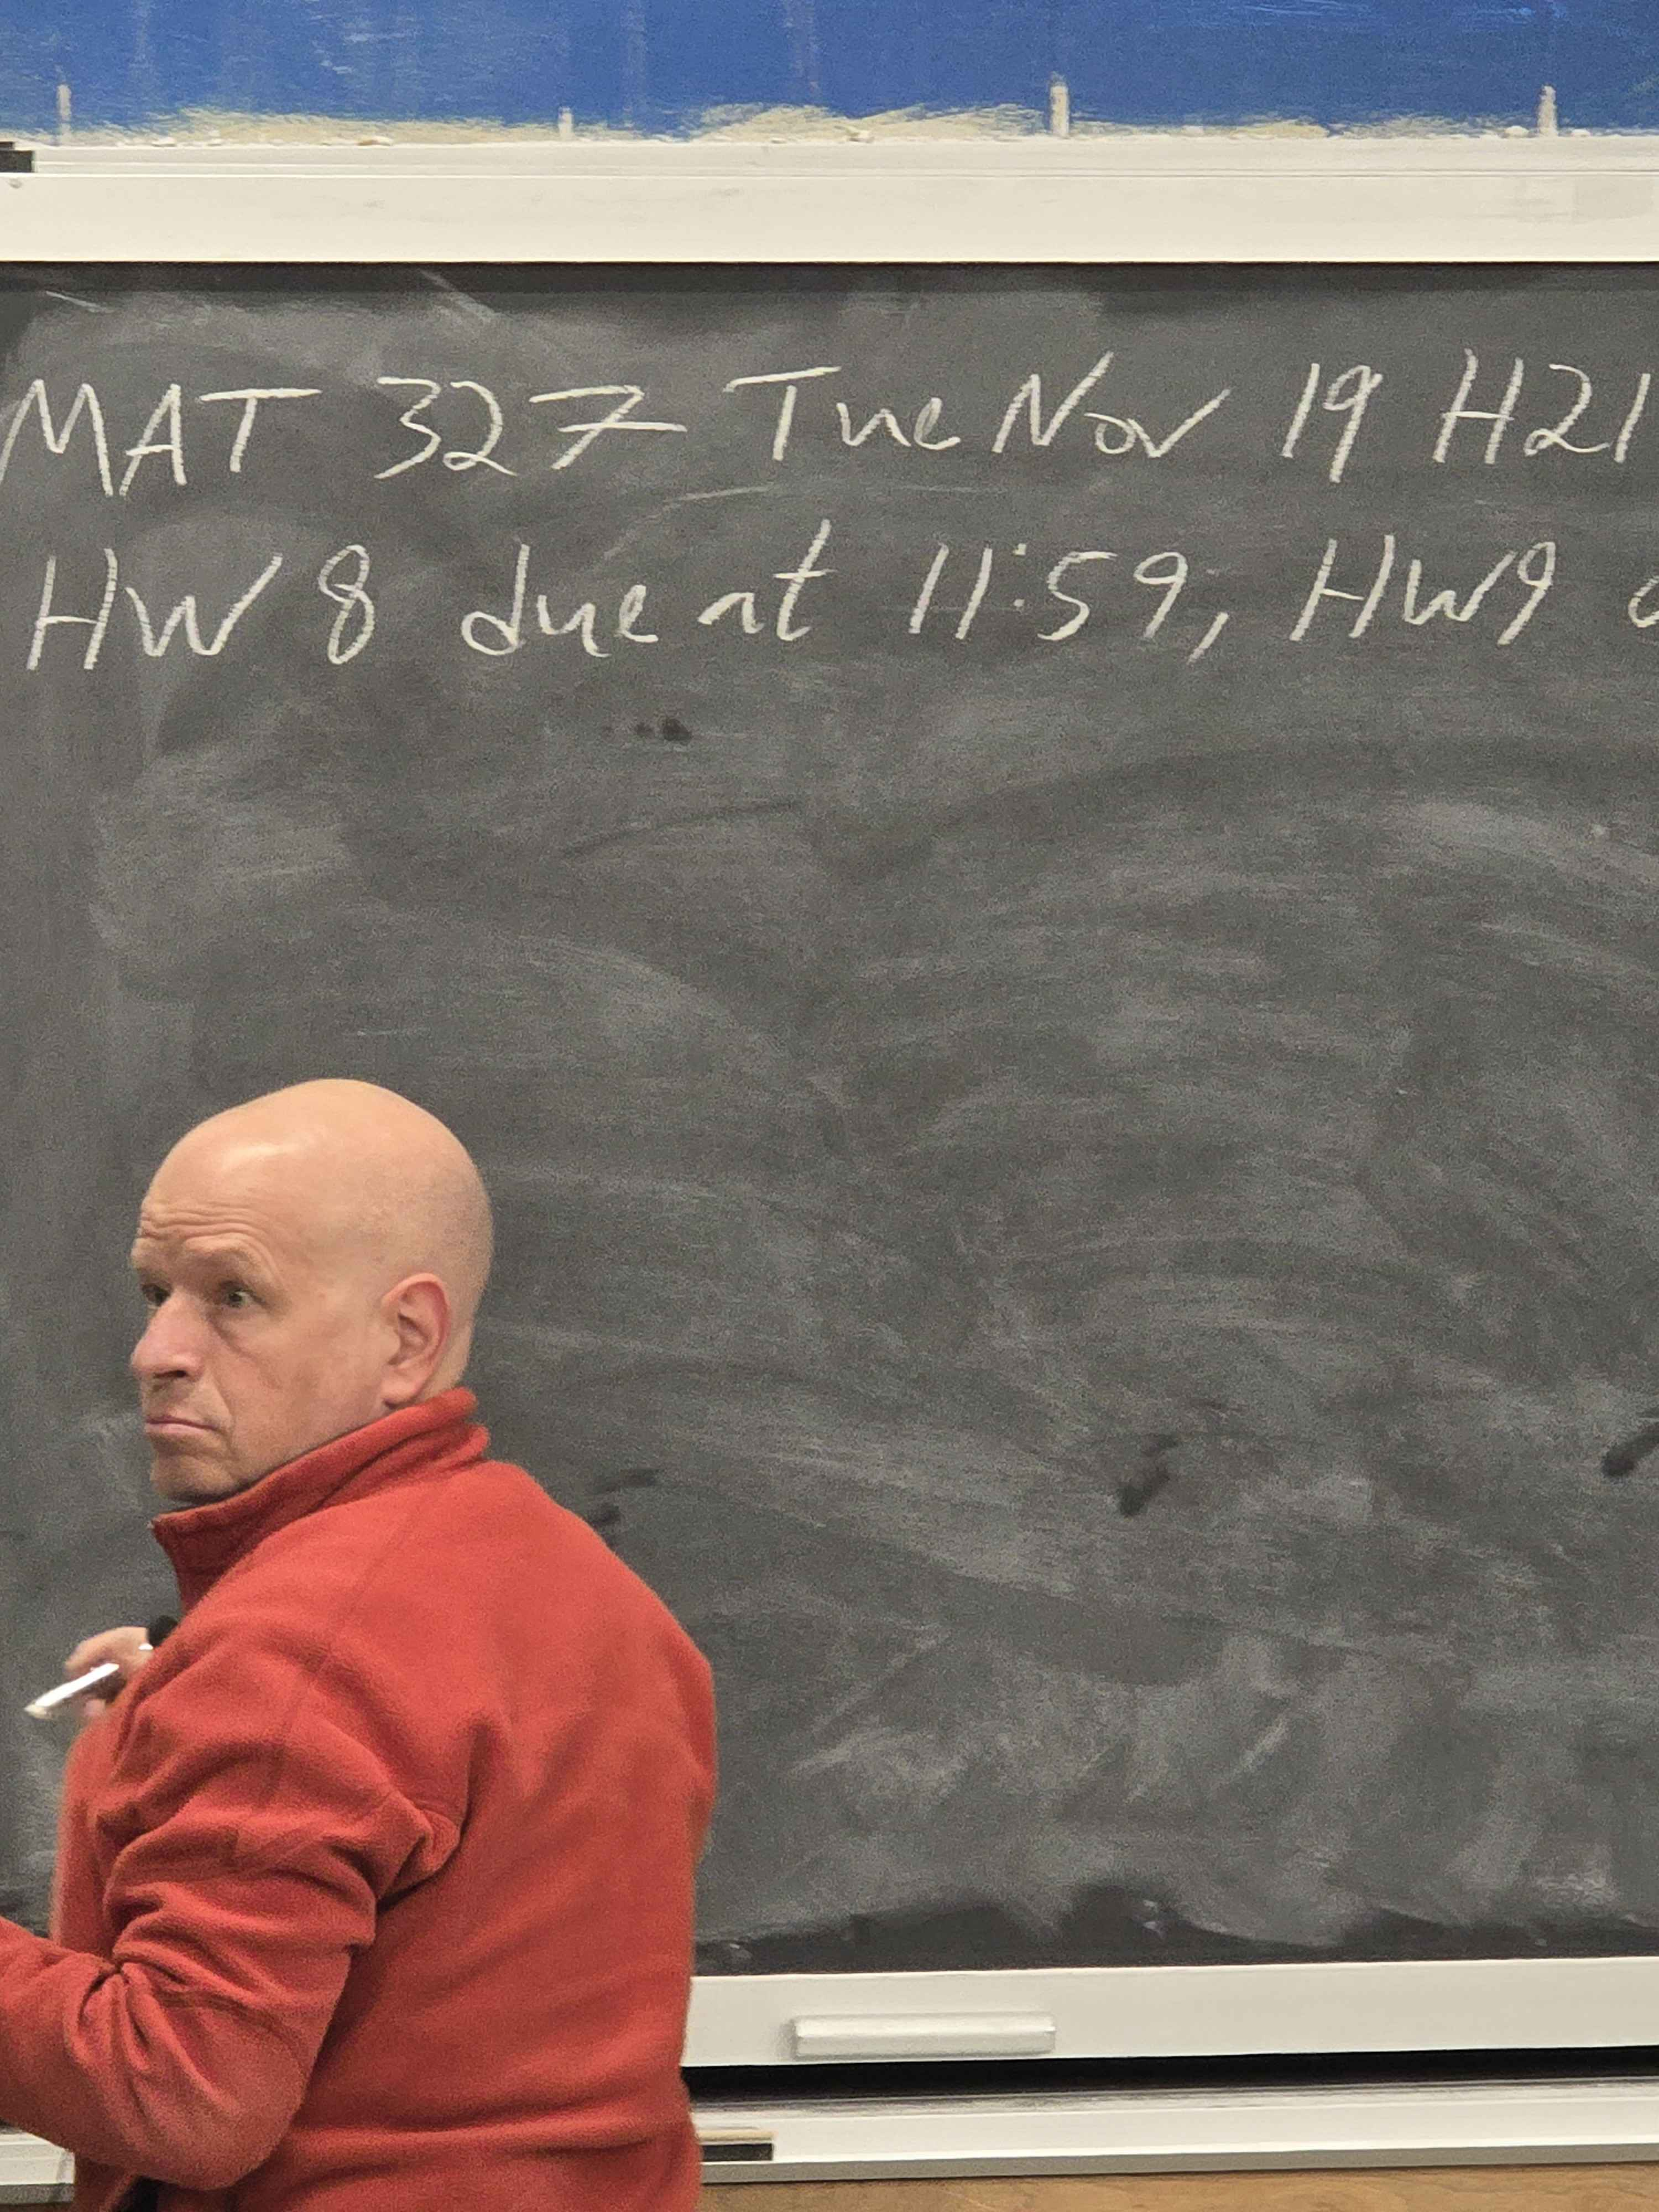
\includegraphics[scale=0.1]{MAT327 Notes/Dror Shirts/dror day 21 shirt.jpg}
\end{figure}

\noindent Recall that the fundamental group, where $(X, x_0)$ is a based space, is given by
\[ \pi_1(X, x_0) = \{[\gamma] \mid \gamma : [0, 1] \to X; \gamma(0) = \gamma(1) = x_0 \}. \]
In particular, $\pi_1(X, x_0)$, as the name suggests is a group; for example, $\pi_1(S^1, 1) \cong \ZZ$. The notation $f : (X, x_0) \to (Y, y_0)$ represents a function $f : X \to Y$ with $f(x_0) = y_0$. If $p : E \to B$ is a covering, it means by $B$ can be covered with open $U_\alpha$ such that, for all $\alpha$, $p^{-1}(U_\alpha)$ is a disjoint union of open sets such that $p$ is a homeomorphism of each of them with $U_\alpha$.
\medskip\newline
An example of a covering space is the map $\RR \to S^1 = \{z \in \CC \mid \abs{z} = 1\}$, where $x \mapsto e^{ix}$.
\begin{simplelemma}
    If $(X, x_0)$ is a connected based space, $p : (E, e_0) \to (B, b_0)$ is a covering, and $\psi : (X, x_0) \to (B, b_0)$ is ``small'', i.e. $\mathrm{Im} (\psi) \subset U_\alpha$, where $U_\alpha$ is as in the definition of a covering, then it has a unique lift $\tilde{\psi} : (X, x_0) \to (E, e_0)$ such that $p \circ \tilde{\psi} = \psi$.
\end{simplelemma}
\noindent $p^{-1}(U_\alpha) = \bigcup_\beta U_{\alpha_\beta}$, where $U_{\alpha_\beta}$ are open in $E$, and $p : U_{\alpha_\beta} \to U_\alpha$ is a homeomorphism for each $\beta$. Only one of $U_{\alpha_\beta}$, say, $U_{\alpha_{\beta_0}}$, contains $e_0$, and we lift $\psi$ to $\tilde{\psi} : (X, x_0) \to (U_{\alpha_{\beta_0}}, e_0)$, using the fact that $U_{\alpha_{\beta_0}}$ is homeomorphic to $U_\alpha$. \qed
\begin{simplethm}[The Path Lifting Property / Lemma 54.1; Munkres]
    Let $p : (E, e_0) \to (B, b_0)$ a covering, $\gamma : (I, 0) \to (B, b_0)$ a path be given; then there exists a unique lift $\tilde{\gamma} : (I, 0) \to (E, e_0)$ such that $p \circ \tilde{\gamma} = \gamma$.
\end{simplethm}
\noindent Let $\{U_\alpha\}$ be an open cover of $B$ such that for all $\alpha$, $p^{-1}(U_\alpha)$ is etc etc etc. then $\{\gamma^{-1}(U_\alpha)\}$ is an open cover of $I$. By the lebesgue covering lemma (since $I$ is compact), there exists $\delta$ such that every subinterval of $I$ of length less than $\delta$ is contained in one of the $\gamma^{-1}(U_\alpha)$'s. Pick $n > \frac{1}{\delta}$ and consider $I = \bigcup I_k$ where $I_k = [\frac{k-1}{n}, \frac{k}{n}]$ for $k = 1, \dots, n$. $\restr{\gamma}{I_k}$ is small in the sense of the previous lemma, and so we can lift $\gamma$ uniquely to $\bigcup_{k=1}^m I_k$ by induction on $m$. \qed

\begin{simplethm}[The Homotopy Lifting Property / Lemma 54.2; Munkres]
    Let $p : (E, e_0) \to (B, b_0)$ be a covering, $H : (I^2, 0) \to (B, b_0)$ be given, then there exists a unique homotopy $\tilde{H} : (I^2, 0) \to (E, e_0)$ such that $p \circ \tilde{H} = H$.
\end{simplethm}
\noindent The proof is the exact same; except in the end, instead of constructing intervals, we have a square instead. Check Munkres p.344 for the diagram. \qed